\chapter{Regularization-based Models}
\label{chapter:regularization}


\begin{chapabstract}
    In this chapter, we propose an overview of regularization in Continual Learning.
    In particular, we discuss regularizations that are applied on the networks' outputs
    and discuss

    The work in this section has led to a publication to a conference paper and a workshop paper:

    \begin{itemize}
        \item \fullcite{douillard2020podnet}
        \item \fullcite{douillard2020ghost}
    \end{itemize}

\end{chapabstract}



\minitoc
\chapterwithfigures{\nameref*{chapter:regularization}}
\chapterwithtables{\nameref*{chapter:regularization}}

\ifthenelse{\boolean{skipRegul}}{\endinput}{}

\section{Introduction}

\ac{CIL}, where each task brings new classes, is among the most challenging setting of \ac{CL}.
When evaluated in single-head, where the task identity is not known at test-time,
the majority of the methods rely on rehearsal learning where a limited amount of old data
is replayed. Furthermore, it is often combined to regularizations that aim to limit
forgetting.


\section{PODNet: reducing forgetting}

\subsection{Model}
\label{sec:podnet_model}


Formally, we learn the model in $T$ \textit{tasks}, task $t$ comprising a set of new classes
$C^t_N$, and a set of old classes $C^t_O$, and aiming at classifying all seen classes $C^t_O \cup
    C^t_N$. Between tasks, the new set $C^t_O$ will be set to $C^{t-1}_O \cup C^{t-1}_N$, but the amount
of training samples from $C^t_O$ (called \textit{memory}) is constrained to exactly $M_\mathrm{per}$
samples per class, while all training samples in the dataset are allowed for the classes in $C^t_N$,
as shown in \autoref{fig:protocol}. The resulting imbalance, if unmanaged, leads to
\textit{catastrophic
    forgetting}~\cite{robins1995catastrophicforgetting,french1999catastrophicforgetting}, i.e., learning
the new classes at the cost of forgetting the old ones.

Our base model is a deep convolutional network $\vyh = g(f(\vx))$, where $\vx$ is the input image,
$\mathbf{y}$ is the output vector of class probabilities, $\vh = f(\vx)$ is the ``feature
extraction'' part of the network (all layers up to the next-to-last), $\vyh = g(\vh)$ is the final
classification layer, and $\vh$ is the final embedding of the network before classification
(\autoref{fig:model}). The superscript $t$ denotes the model learned at task $t$:$f^{t}$, $g^{t}$,
$\vh^{t}$, etc.


\subsubsection{POD: Pooled Outputs Distillation loss}
\label{sec:pod}

Constraining the evolution of the weights is crucial to reduce forgetting. Each new task $t$ learns
a new (student) model, whose weights are not only initialized with those of the previous (teacher)
model, but also constrained by a distillation loss. That loss must be carefully balanced to prevent
forgetting (rigidity), while allowing the learning of new classes (plasticity).

To this goal, we propose a set of constraints we call \textbf{Pooled Outputs Distillation (POD)},
applied not only over the final embedding output by $\vh^{t}=f^{t}(\vx)$, but also over the output
of its intermediate layers $\vh^{t}_\ell=f^{t}_\ell(\vx)$ (where by notation overloading
$f^{t}_\ell(\vx)\equiv f^{t}_\ell\circ\ldots\circ f^{t}_1(\vx)$, and thus $f^{t}(\vx)\equiv
    f^{t}_L\ldots\circ f^{t}_\ell\circ\ldots f^{t}_1(\vx)$).

The convolutional layers of the network output tensors $\vh^{t}_{\ell}$ with components
$\vh^{t}_{\ell,c,w,h}$, where $c$ stands for channel (filter), and $w\times h$ for column and row of
the spatial coordinates. The loss used by POD may pool (sum over) one or several of those indexes,
more aggressive poolings (\autoref{fig:pooling}) providing more freedom, and thus, plasticity: the
lowest possible plasticity imposes an exact similarity between the previous and current model while
higher plasticity relaxes the similarity definition.

Pooling is an important operation in Computer Vision, with a strong theoretical motivation. In the
past, pooling has been introduced to obtain invariant
representations~\cite{lowe1999sift,lazbnik2006spatial_pyramid_matching}. Here, the justification is
similar, but the goal is different: as we will see, the pooled indexes are aggregated in the
proposed loss, allowing \textit{plasticity}. Instead of the model acquiring invariance to the input
image, the desired loss acquires invariance to model evolution, and thus, representation.
%
The proposed pooling-based formalism has two advantages: first, it organizes disparately proposed
distillation losses into a neat, general formalism. Second, as we will see, it allowed us to propose
novel distillation losses, with better plasticity-rigidity compromises. Those topics are explored
next.

\begin{figure}[tb]
    \begin{center}
        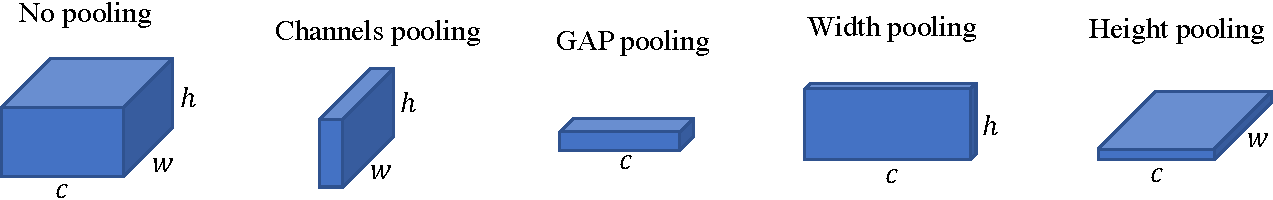
\includegraphics[width=0.90\linewidth]{images/podnet/pooling}
    \end{center}
    \caption{\textbf{Different possible poolings}. The output from a convolutional layer
        $\vh^{t}_{\ell,c,w,h}$ may be pooled (summed over) one or more axes. The resulting loss
        considers only the pooled activations instead of the individual components, allowing more
        plasticity across the pooled axes.}
    \label{fig:pooling}
\end{figure}

\paragraph{Pooling of convolutional outputs} As explained before, POD constrains the output of each
intermediate convolutional layer $\vh^{t}_{\ell,c,w,h} = f^{t}_\ell(\cdot)$ (in practice, each stage
of a ResNet~\cite{he2016resnet}). As a reminder, $c$ is the channel and $w\times h$ are the spatial
coordinates. All POD variants use the Euclidean distance of $\ell^2$-normalize tensors, here noted
as $\left\Vert\cdot-\cdot\right\Vert$. They differ on the type of pooling applied before that
distance is computed.
%
On one extreme, one can apply no pooling at all, resulting in the most strict loss, the most rigid
constrains, and the lowest plasticity:
%
\begin{equation}
    \mcL_{\text{POD-pixel}}(\vh^{t-1}_\ell, \vh^t_\ell) = \sum_{c=1}^C \sum_{w=1}^{W} \sum_{h=1}^{H} \left\Vert \vh^{t-1}_{\ell,c,w,h} - \vh^t_{\ell,c,w,h} \right\Vert^2\label{eq:pod_pixel}\,.
\end{equation}
%
By pooling the channels, one preserves only the spatial coordinates, resulting in a more permissive
loss, allowing the activations to reorganize across the channels, but penalizing global changes of
those activations across the space,
%
\begin{equation}
    \mcL_{\text{POD-channel}}(\vh^{t-1}_\ell, \vh^t_\ell)  = \sum_{w=1}^{W} \sum_{h=1}^{H} \left\Vert \sum_{c=1}^C \vh^{t-1}_{\ell,c,w,h} - \sum_{c=1}^C \vh^{t}_{\ell,c,w,h} \right\Vert^2\label{eq:pod_channel}\,;
\end{equation}
%
or, contrarily, by pooling the space (equivalent, up to a factor, to a Global Average Pooling), one
preserves \textit{only} the channels:
%
\begin{equation}
    \mcL_{\text{POD-gap}}(\vh^{t-1}_\ell, \vh^t_\ell) = \sum_{c=1}^{C} \left\Vert \sum_{w=1}^{W} \sum_{h=1}^H \vh^{t-1}_{\ell,c,w,h} - \sum_{w=1}^{W} \sum_{h=1}^H \vh^{t}_{\ell,c,w,h} \right\Vert^2\label{eq:pod_gap}\,.
\end{equation}
%

Note that the only difference between the variants is in the position of the summation. For example,
contrast equations \autoref{eq:pod_pixel} and \ref{eq:pod_channel}: in the former the differences
are computed between activation pixels, and then totaled; in the latter, first the channel axis is
flattened, then the differences are computed, resulting in a more permissive loss.

We can trade a little plasticity for rigidity, with less aggressive pooling by aggregating
statistics across just one of the spatial dimensions:
%
\begin{equation}
    \mcL_{\text{POD-width}}(\vh^{t-1}_\ell, \vh^t_\ell)  = \sum_{c=1}^{C} \sum_{h=1}^{H} \left\Vert \sum_{w=1}^W \vh^{t-1}_{\ell,c,w,h} - \sum_{w=1}^W \vh^{t}_{\ell,c,w,h} \right\Vert^2\label{eq:pod_width}\,;
\end{equation}
%
or, likewise, for the vertical dimension, resulting in POD-height. Each of those variants measure
the distribution of activation pixels across their respective axis. These two complementary
intermediate statistics can be further combined together:
%
\begin{equation}
    \mcL_{\text{POD-spatial}}(\vh^{t-1}_\ell, \vh^t_\ell) = \mcL_{\text{POD-width}}(\vh^{t-1}_\ell, \vh^t_\ell) + \mcL_{\text{POD-height}}(\vh^{t-1}_\ell, \vh^t_\ell)\,.
\end{equation}
%
$\mcL_{\text{POD-spatial}}$ is minimal when the average statistics over the dataset, on both width
and height axes, are similar for the previous and current model. It brings the right balance between
being too rigid (\autoref{eq:pod_pixel}) and being too permissive (\autoref{eq:pod_channel} and
\ref{eq:pod_gap}).

\label{sec:pod_flat}
\paragraph{Constraining the final embedding} After the convolutional layers, the network, by design,
flattens the spatial coordinates, and the formalism above needs adjustment, as a summation over $w$
and $h$ is no longer possible. Instead, we set a flat constraint on the final embedding $\vh^{t} =
    f^{t}(\vx)$:
%
\begin{equation}
    \mcL_{\text{POD-flat}}(\vh^{t-1}, \vh^t) = \left\Vert \vh^{t-1} - \vh^t \right\Vert^2\label{eq:POD-flat}\,.
\end{equation}

\paragraph{Combining the losses, analysis} The final POD loss combines the two  components:
%
\begin{multline}
    \mcL_\text{POD-final}(\vx) =  \frac{\lambda_{c}}{L-1}\sum_{\ell=1}^{L-1}  \mcL_{\text{POD-spatial}}\left(f^{t-1}_\ell(\vx), f^t_\ell(\vx)\right) + \\[-0.8em]
    \lambda_{f} \mcL_\text{POD-flat}\left(f^{t-1}(\vx), f^t(\vx)\right)\,.
\end{multline}
%
The hyperparameters $\lambda_{c}$ and $\lambda_{f}$ are necessary to balance the two terms, due to
the  different nature of the intermediate outputs (spatial and flat).

As mentioned, the strategy above generalizes disparate propositions existing both in the literature
of incremental learning, and elsewhere. When $\lambda_{c}=0$, it reduces to the cosine constraint of
\textit{Less-Forget}, proposed by Hou et al. for incremental learning, which constrains only the
final embedding~\cite{hou2019ucir}. When $\lambda_{f}=0$ and POD-spatial is replaced by POD-pixel,
it suggests the Perceptual Features loss, proposed for style
transfer~\cite{johnson2016perceptual_losses}. When $\lambda_{f}=0$ and POD-spatial is replaced by
POD-channel, the strategy hints at the loss proposed by Komodakis et
al.~\cite{komodakis2017attention_residual_distillation} to allow distillation across different
networks, a situation in which the channel pooling responds to the very practical need to allow the
comparison of architectures with different number of channels.

As we will see in our evaluations of pooling strategies (\autoref{sec:ablation_pooling}), what
proved optimal was a completely novel idea, POD-spatial, combining two poolings, each of which
flattens one of the spatial coordinates. That relatively rigid strategy (channels and one of the
spatial coordinates are considered in each half of the loss) makes intuitive sense in our context,
which is \textit{small-task} incremental learning, and thus where we expect a slow drift of the
model across a single task.

% ------------------------------------------------------------

\begin{figure}[t]
    \begin{center}
        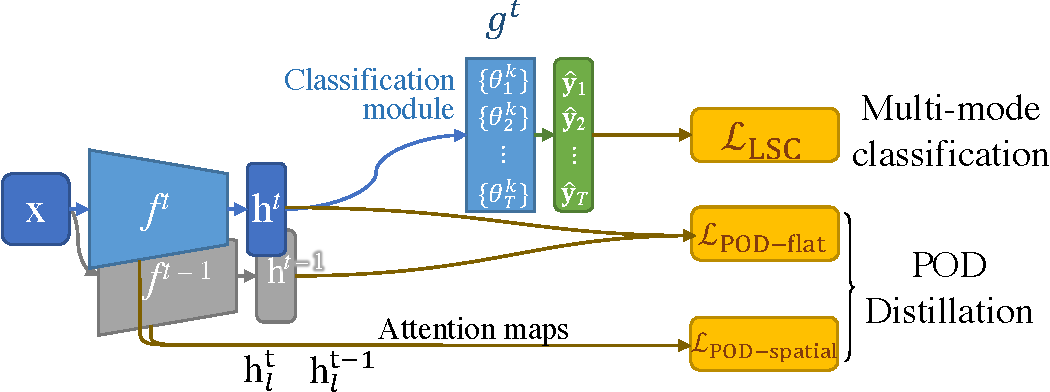
\includegraphics[width=0.8\linewidth]{images/podnet/model}
    \end{center}
    \caption{\textbf{Overview of PODNet}: the distillation loss POD prevent excessive model drift by
        constraining intermediate outputs of the ConvNet $f$ and the LSC classifier $g$ learns a
        more expressive multi-modal representation.}
    \label{fig:model}
\end{figure}

\subsubsection{Local Similarity Classifier}
\label{sec:local_classifier}

Hou et al.~\cite{hou2019ucir} observed that the class imbalance of incremental learning have
concrete manifestations on the parameters of the final layer on classifiers, namely the weights for
the over-represented (new) classes becoming much larger than those for the underrepresented (old)
classes. To overcome this issue, their method (called here UCIR) $\ell^2$-normalizes both the
weights and the activations, which corresponds to taking the cosine similarity instead of the dot
product. For each class $c$, their last layer becomes
%
\begin{equation}
    \vyh_{c}=\frac{\exp\left(\eta\langle\theta_{c},\vh\rangle\right)}{\sum_{i} \exp \left(\eta\langle\theta_{i}, \vh\rangle\right)}\,,
\end{equation}
%
where $\theta_c$ are the last-layer weights for class $c$, $\eta$ is a learned scaling parameter,
and $\langle\cdot,\cdot\rangle$ is the cosine similarity.

However, this strategy optimizes a \textit{global similarity}: its training objective increases the
similarity between the extracted features and their associated weights. For each class, the
normalized weight vector acts as a \textit{single} proxy~\cite{attias2017proxynca}, towards which
the learning procedure pushes all samples in the class.

We observed that such global strategy is hard to optimize in an incremental setting. To avoid
forgetting, the distillation losses (\autoref{sec:distillation}) tries to keep the final embedding
$\vh$ consistent through time so that the class proxies stay relevant for the classifier.
Unfortunately catastrophic forgetting, while alleviated by current methods, is not solved and thus
the distribution of $\vh$ may change. The cosine classifier is very sensitive to those changes as it
models a unique majority mode through its class proxies.


\paragraph{Local Similarity Classifier} The problem above lead us to amend the classification layer
during training, in order to consider multiple proxies/modes per class. A shift in the distribution
of $\vh$ will have less impact on the classifier as more modes are covered.


Our redesigned classification layer, which we call Local Similarity Classifier (LSC), allows for $K$
multiple proxies/modes during training. Like before, the proxies are a way to interpret the weight
vector in the cosine similarity, thus we allow for $K$ vectors $\theta_{c,k}$ for each class $c$.
The similarity $s_{c,k}$ to each proxy/mode is first computed. An averaged class similarity $\vyh_c$
is the output of the classification layer:
%
\begin{equation}
    s_{c,k} =\frac{\exp\,\langle\theta_{c,k},\vh\rangle}{\sum_{i} \exp\,\langle\theta_{c,i},\vh\rangle}\,, \qquad
    \vyh_c = \sum_{k}s_{c,k}\,\langle\theta_{c,k},\vh\rangle\,.
\end{equation}
%
The multi-proxies classifier optimizes the similarity of each sample to its ground truth class
representation and minimizes all others. A simple cross-entropy loss would work, but we found
empirically that the NCA loss~\cite{goldberger2005nca_loss,attias2017proxynca} converged faster. We
added to the original loss a hinge $[\,\cdot\,]_+$ to keep it bounded, and a small margin $\delta$
to enforce stronger class separation, resulting in the final formulation:
%
\begin{equation}
    \mcL_\text{LSC} = \left[- \log\frac{\exp\left(\eta (\vyh_y - \delta)\right)}{\sum_{i \neq y} \exp \eta \vyh_{i}} \right]_+ \,.
\end{equation}

\paragraph{Weight initialization for new classes} The incremental learning setting imposes detecting new
classes at each new task $t$. New weights $\{\theta_{c,k} \mid \forall c \in C^t_N, \forall k \in
    {1...K}\}$ must be added to predict them. We could initialize them randomly, but the class-agnostic
features of the ConvNet $f$, extracted by the model trained so far offer a better prior. Thus, we
employ a generalization of Imprinted Weights~\citep{qi2018imprintedweights} procedure to multiple
modes: for each new class $c$, we extract the features of its training samples, use a k-means
algorithm to split them into $K$ clusters, and use the centroids of those clusters as initial values
for $\theta_{c,k}$. This procedure ensures mode diversity at the beginning of a new task and
resulted in a one percentage point improvement on CIFAR100.

% ------------------------------------------------------------

\subsubsection{Complete model formulation}

Our model has the classical structure of a convolutional network $f(\cdot)$ acting as a feature
extractor, and a classifier $g(\cdot)$ producing a score per class. We introduced two innovations to
this model: (1) our main contribution is a novel distillation loss (POD) applied all over the
ConvNet, from the spatial features $\vh_\ell$ to the final flat embedding $\vh$; (2) as further
refinement we propose that the classifier learns a multi-modal representation that explicitly keeps
multiple proxy vectors per class, increasing the model expressiveness and thus making it less
sensible to shift in the distribution of $\vh$. The final loss for current model $g^t \circ f^t$,
i.e., the model trained for task $t$, is simply their addition $\mathcal{L}_{\{f^t; g^t\}} =
    \mathcal{L}_\textrm{LSC} + \mathcal{L}_\textrm{POD-final}$.

\subsection{Experiment results}

\paragraph{Datasets} CIFAR100 \citep{krizhevskycifar100}, ImageNet \citep{deng2009imagenet}


\section{Ghost: avoid pre-emptively forgetting}

\subsection{Prescient Continual Learning}

\subsection{Model}

\subsection{Experiment results}


\section{Conclusion}

